\chapter{Caso studio illustrativo}
\label{chap:caso-studio}

Il presente capitolo applica i concetti introdotti nel Capitolo~\ref{cap:quadro_teorico} a un caso studio concreto, costruito sul dataset pubblico \emph{IBM HR Employee Attrition}. L'obiettivo non è produrre un contributo sperimentale originale, ma mostrare in modo operativo come i tre framework discussi --- SHAP, LIME e controfattuali Alibi --- si comportino quando applicati allo stesso modello e alle stesse istanze. La coerenza del protocollo sperimentale è dunque funzionale a un confronto qualitativo tra i diversi tipi di spiegazione, non a una valutazione quantitativa delle prestazioni del modello.

\section{Dataset e setup}
\label{sec:dataset_setup}

\subsection{Il dataset IBM HR Attrition}

Il dataset è costituito da \num{1470} record, ciascuno relativo a un dipendente, descritti da \num{35} variabili di natura eterogenea (anagrafiche, retributive, di ruolo, di soddisfazione e di tenure). La variabile target è \texttt{Attrition}, binaria, che indica se il dipendente ha lasciato l'azienda. La distribuzione del target è fortemente sbilanciata: \num{1233} dipendenti (83{,}9\%) risultano rimasti in azienda e \num{237} (16{,}1\%) hanno abbandonato, come illustrato in Figura~\ref{fig:eda_class_balance}. Tale sbilanciamento condiziona tanto la scelta della metrica di valutazione quanto la strategia di bilanciamento in fase di training.

\begin{figure}[htbp]
    \centering
    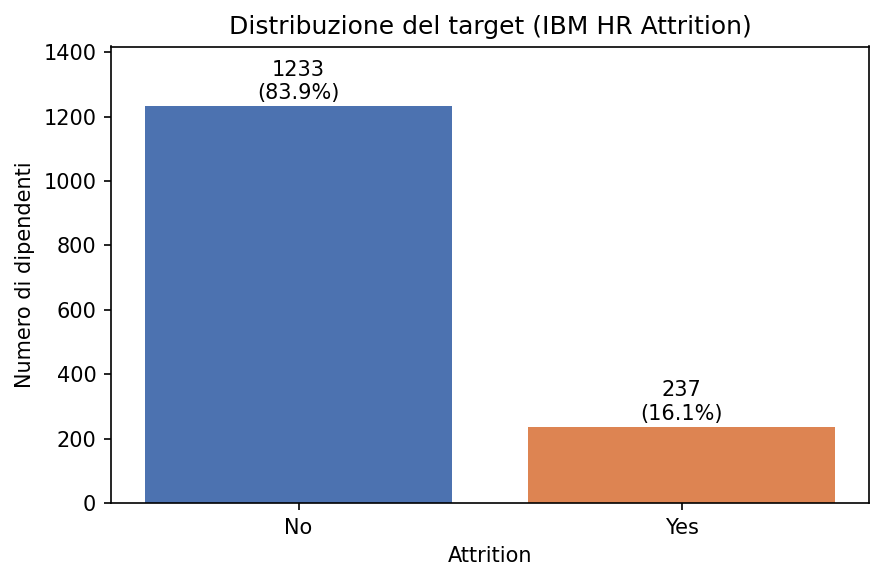
\includegraphics[width=0.7\textwidth]{media/eda_class_balance.png}
    \caption{Distribuzione del target \texttt{Attrition}: il dataset è fortemente sbilanciato, con una classe positiva (dipendenti che hanno abbandonato) pari al 16{,}1\% del totale.}
    \label{fig:eda_class_balance}
\end{figure}

L'analisi esplorativa preliminare ha prodotto due osservazioni utili alla contestualizzazione dei risultati successivi. La prima riguarda la relazione tra età e abbandono: come mostrato in Figura~\ref{fig:eda_age_vs_attrition}, la distribuzione dell'età nel gruppo di dipendenti in uscita è spostata verso valori inferiori, suggerendo che i profili più giovani presentino una propensione relativa maggiore al turnover. La seconda osservazione riguarda la matrice di correlazione tra le feature numeriche (Figura~\ref{fig:eda_correlation_heatmap}): emerge un blocco di forti correlazioni tra le variabili di tenure (\texttt{YearsAtCompany}, \texttt{YearsInCurrentRole}, \texttt{YearsSinceLastPromotion}, \texttt{YearsWithCurrManager}), coerenti con il fatto di misurare tutte dimensioni temporali legate alla permanenza nell'organizzazione. Una correlazione elevata è presente anche tra \texttt{JobLevel}, \texttt{MonthlyIncome} e \texttt{TotalWorkingYears}, aspetto rilevante per l'interpretazione delle spiegazioni locali: SHAP e LIME potrebbero attribuire quote di importanza a feature che, dal punto di vista causale, sono manifestazioni del medesimo costrutto sottostante.

\begin{figure}[htbp]
    \centering
    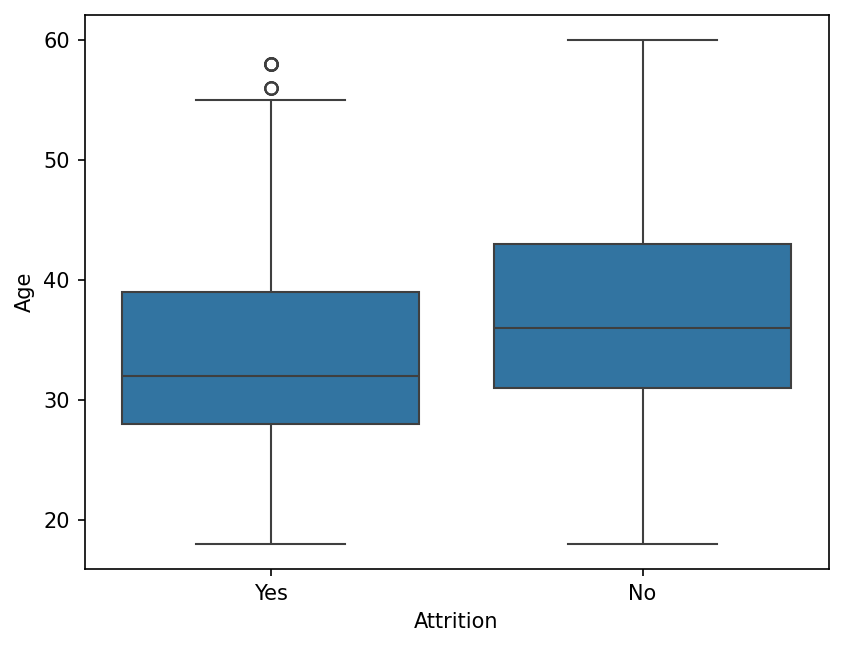
\includegraphics[width=0.65\textwidth]{media/eda_age_vs_attrition.png}
    \caption{Distribuzione dell'età rispetto al target: la mediana dei dipendenti in uscita risulta inferiore rispetto a quella di chi è rimasto, indicando una maggiore propensione all'abbandono tra i profili più giovani.}
    \label{fig:eda_age_vs_attrition}
\end{figure}

\begin{figure}[htbp]
    \centering
    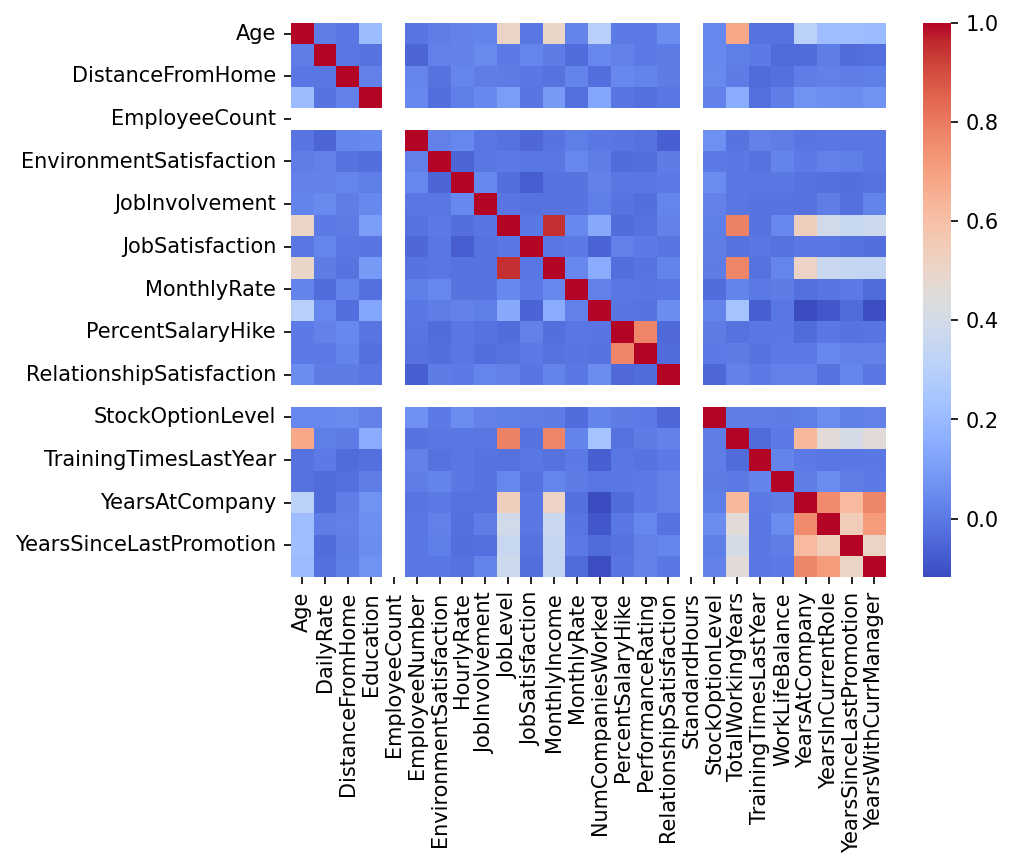
\includegraphics[width=0.85\textwidth]{media/eda_correlation_heatmap.png}
    \caption{Heatmap di correlazione tra le feature numeriche. Sono evidenti i blocchi di alta correlazione tra le variabili di tenure e tra \texttt{JobLevel}, \texttt{MonthlyIncome} e \texttt{TotalWorkingYears}.}
    \label{fig:eda_correlation_heatmap}
\end{figure}

\subsection{Preprocessing}

Il preprocessing è stato mantenuto volutamente minimale per evitare di introdurre trasformazioni che ostacolino l'interpretabilità delle spiegazioni locali. In particolare:

\begin{itemize}
    \item sono state rimosse le feature costanti o identificative (\texttt{EmployeeCount}, \texttt{Over18}, \texttt{StandardHours}, \texttt{EmployeeNumber}), prive di potere discriminante;
    \item il target \texttt{Attrition} è stato codificato come binario (\texttt{Yes} $\mapsto 1$, \texttt{No} $\mapsto 0$);
    \item le variabili categoriche sono state trasformate mediante one-hot encoding con \texttt{drop\_first=True}, per evitare la collinearità perfetta della codifica dummy;
    \item le variabili numeriche sono state lasciate nella loro scala originale, poiché XGBoost, basandosi su split binari degli alberi, non richiede standardizzazione.
\end{itemize}

A valle di queste operazioni il numero di feature passa da \num{35} a \num{44}, rimanendo compatibile con un training efficiente e con la leggibilità delle spiegazioni locali. Il dataset è stato quindi suddiviso in train e test con proporzione 80/20, stratificando rispetto al target e fissando \texttt{random\_state=42} per garantire la riproducibilità.

\subsection{Strategia di bilanciamento e tuning degli iperparametri}

Date le caratteristiche del dataset, l'indicatore di prestazione principale è l'\emph{F1-score} sulla classe positiva, che bilancia precision e recall e risulta più informativo dell'accuracy in presenza di classi sbilanciate. Sono state confrontate due strategie di bilanciamento:

\begin{itemize}
    \item \textbf{SMOTE} (Synthetic Minority Over-sampling Technique), inserito all'interno di una pipeline \texttt{imblearn} in modo da essere applicato solo sui fold di training all'interno della cross-validation, evitando data leakage;
    \item \textbf{scale\_pos\_weight}, parametro nativo di XGBoost che aumenta il peso degli errori sulla classe positiva nella funzione di loss, calibrato come rapporto tra le frequenze delle due classi sul train.
\end{itemize}

Entrambe le strategie sono state accoppiate a una \texttt{RandomizedSearchCV} con \num{150} iterazioni, \texttt{StratifiedKFold} a \num{5} fold e scoring \texttt{f1}. Lo spazio di ricerca degli iperparametri, identico nelle due configurazioni, è riportato in forma compatta in Tabella~\ref{tab:hyperparam_space} e in forma estesa in appendice~\ref{app:hyperparam}.

\begin{table}[htbp]
    \centering
    \caption{Spazio di ricerca degli iperparametri di XGBoost (sintesi).}
    \label{tab:hyperparam_space}
    \begin{tabular}{ll}
        \toprule
        Iperparametro & Valori esplorati \\
        \midrule
        \texttt{n\_estimators}    & 100, 200, 300, 500, 700 \\
        \texttt{max\_depth}       & 3, 4, 5, 6, 7, 8 \\
        \texttt{learning\_rate}   & 0.01, 0.03, 0.05, 0.08, 0.1, 0.15 \\
        \texttt{subsample}        & 0.6, 0.7, 0.8, 0.9, 1.0 \\
        \texttt{colsample\_bytree}& 0.5, 0.6, 0.7, 0.8, 0.9, 1.0 \\
        \texttt{min\_child\_weight}& 1, 2, 3, 5, 7 \\
        \texttt{gamma}            & 0, 0.05, 0.1, 0.2, 0.3 \\
        \texttt{reg\_alpha}       & 0, 0.001, 0.01, 0.1, 1.0 \\
        \texttt{reg\_lambda}      & 0.5, 1.0, 1.5, 2.0, 3.0 \\
        \bottomrule
    \end{tabular}
\end{table}

Il confronto tra le due strategie, effettuato sul medesimo seed di cross-validation, ha selezionato \texttt{scale\_pos\_weight} come configurazione vincente in termini di F1 sul test set. Oltre al vantaggio metrico, tale scelta presenta due vantaggi rilevanti per il caso studio: non altera le istanze di training (i controfattuali Alibi useranno quindi un manifold non contaminato da dati sintetici) e semplifica la pipeline, eliminando l'oversampling esterno. Il modello finale è dunque un XGBoost classifier con \texttt{scale\_pos\_weight} calibrato e gli iperparametri ottimali individuati dalla ricerca randomizzata; gli artefatti prodotti sono il modello serializzato (\texttt{models/xgb\_model.ubj}) e i dataset pickle di train e test, utilizzati nei notebook di spiegazione per garantire coerenza tra le analisi.

\section{Performance del modello}
\label{sec:performance}

Le metriche ottenute dal modello finale sul test set, a soglia di classificazione predefinita (\num{0.50}), sono riportate in Tabella~\ref{tab:metrics_default}. Il test set è composto da \num{294} istanze, di cui \num{247} appartenenti alla classe negativa (dipendenti rimasti) e \num{47} alla classe positiva (dipendenti usciti).

\begin{table}[htbp]
    \centering
    \caption{Prestazioni del modello XGBoost sul test set (soglia $=0{,}50$).}
    \label{tab:metrics_default}
    \begin{tabular}{lc}
        \toprule
        Metrica & Valore \\
        \midrule
        Accuracy    & 0{,}823 \\
        Precision   & 0{,}456 \\
        Recall      & 0{,}553 \\
        F1-score    & 0{,}500 \\
        AUC-ROC     & 0{,}801 \\
        \bottomrule
    \end{tabular}
\end{table}

L'accuracy dell'82{,}3\% è poco al di sopra della baseline banale del classificatore che predice sempre la classe maggioritaria (circa 83{,}9\%, coincidente con la frequenza della classe negativa), e per questo motivo è una metrica poco informativa in questo contesto. L'informazione rilevante è contenuta nella coppia precision/recall e nella AUC-ROC. In particolare, recall e precision sulla classe positiva ($0{,}553$ e $0{,}456$) indicano che il modello individua circa la metà dei dipendenti che effettivamente abbandoneranno, accettando in cambio un tasso di falsi positivi non trascurabile. L'AUC-ROC pari a $0{,}801$ conferma che, indipendentemente dalla soglia, il modello è in grado di separare le due classi in modo nettamente migliore del caso ($0{,}500$).

\begin{figure}[htbp]
    \centering
    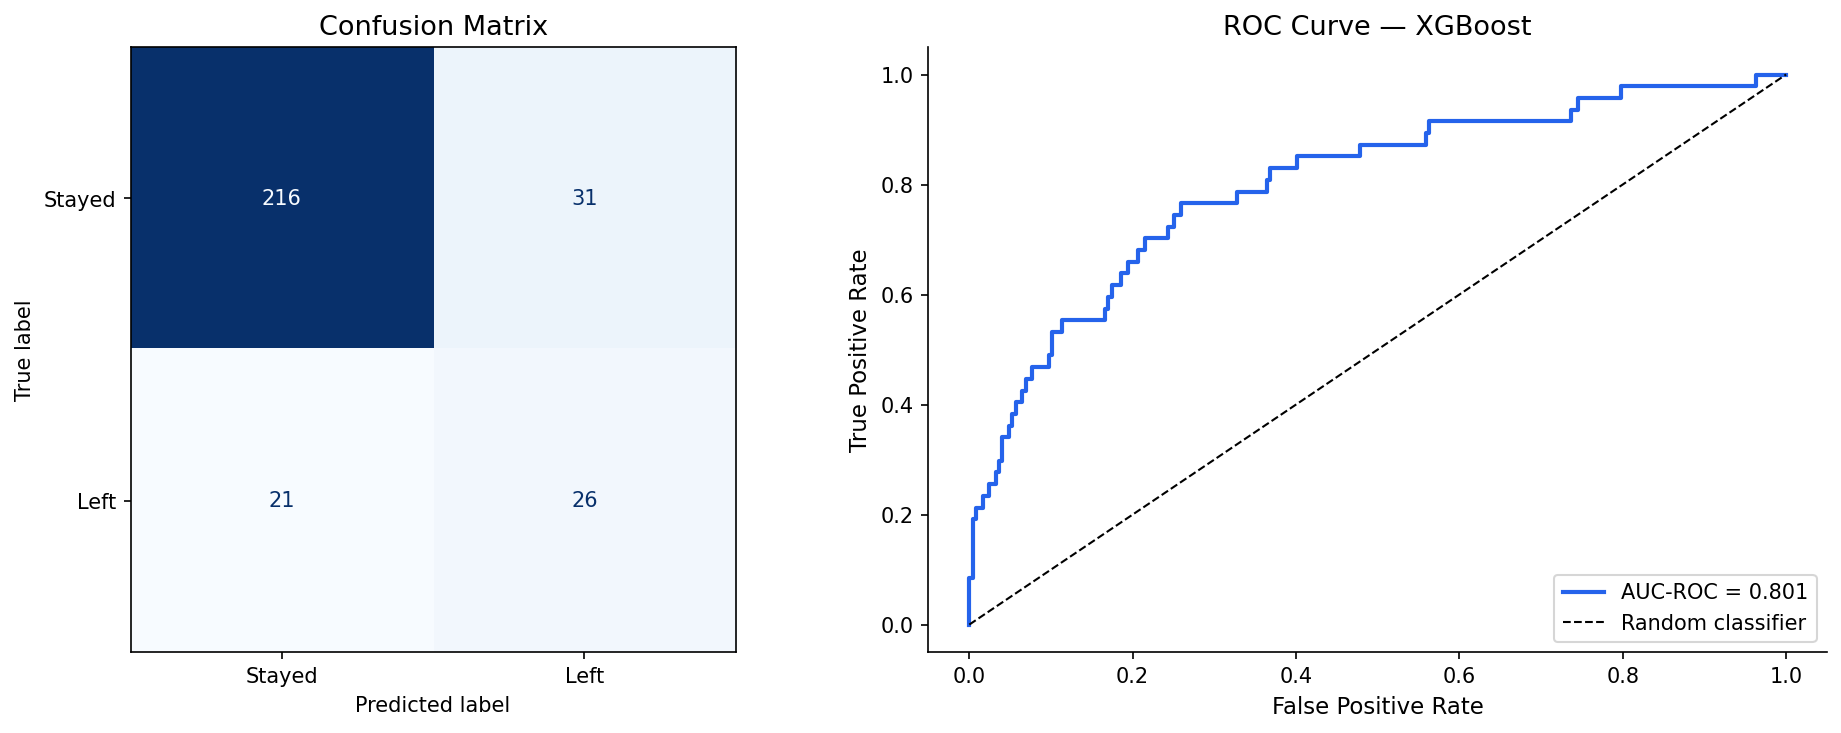
\includegraphics[width=\textwidth]{media/model_metrics.png}
    \caption{Matrice di confusione (sinistra) e curva ROC (destra) sul test set a soglia $=0{,}50$.}
    \label{fig:model_metrics}
\end{figure}

La matrice di confusione in Figura~\ref{fig:model_metrics} rende esplicita la distribuzione degli errori. Il modello commette errori di entrambi i tipi, ma il dato significativo dal punto di vista organizzativo è il numero di \emph{falsi negativi}, cioè di dipendenti realmente in uscita che il modello ha classificato come stabili. Questi casi rappresentano l'oggetto di interesse prioritario per un responsabile HR, perché corrispondono a situazioni in cui il sistema \emph{non segnala} un rischio che è invece presente: è lì che lo strumento predittivo perde utilità.

\subsection{Ottimizzazione della soglia}

L'asimmetria nel costo degli errori suggerisce di non utilizzare la soglia predefinita $0{,}50$, che bilancia in modo simmetrico precision e recall, ma di spostarla in modo da privilegiare il recall. Dal punto di vista dell'azienda, infatti, un falso positivo (intervenire in via precauzionale su un dipendente che sarebbe rimasto comunque) ha un costo contenuto, riconducibile al tempo speso dall'HR manager e, al più, a un incentivo non necessario. Un falso negativo, al contrario, significa non cogliere un segnale di rischio: il costo include il turnover effettivo, la ricerca del sostituto, l'onboarding e la perdita di capitale umano. Non è quindi ragionevole assumere i due errori come equiparabili.

La Figura~\ref{fig:threshold_optimization} mostra a sinistra la curva precision--recall del modello e a destra l'andamento di precision, recall e F1 al variare della soglia di classificazione. Sono state confrontate tre soglie:

\begin{itemize}
    \item \textbf{Soglia predefinita} ($t=0{,}50$): la configurazione standard di \texttt{predict}, presentata sopra.
    \item \textbf{Soglia che massimizza F1} ($t \approx 0{,}52$): punto di ottimo rispetto alla metrica di tuning, con uno scostamento minimo rispetto al default.
    \item \textbf{Soglia business-oriented} ($t \approx 0{,}38$): scelta per garantire un recall non inferiore al \num{66}\%, a scapito di una precision più bassa.
\end{itemize}

\begin{figure}[htbp]
    \centering
    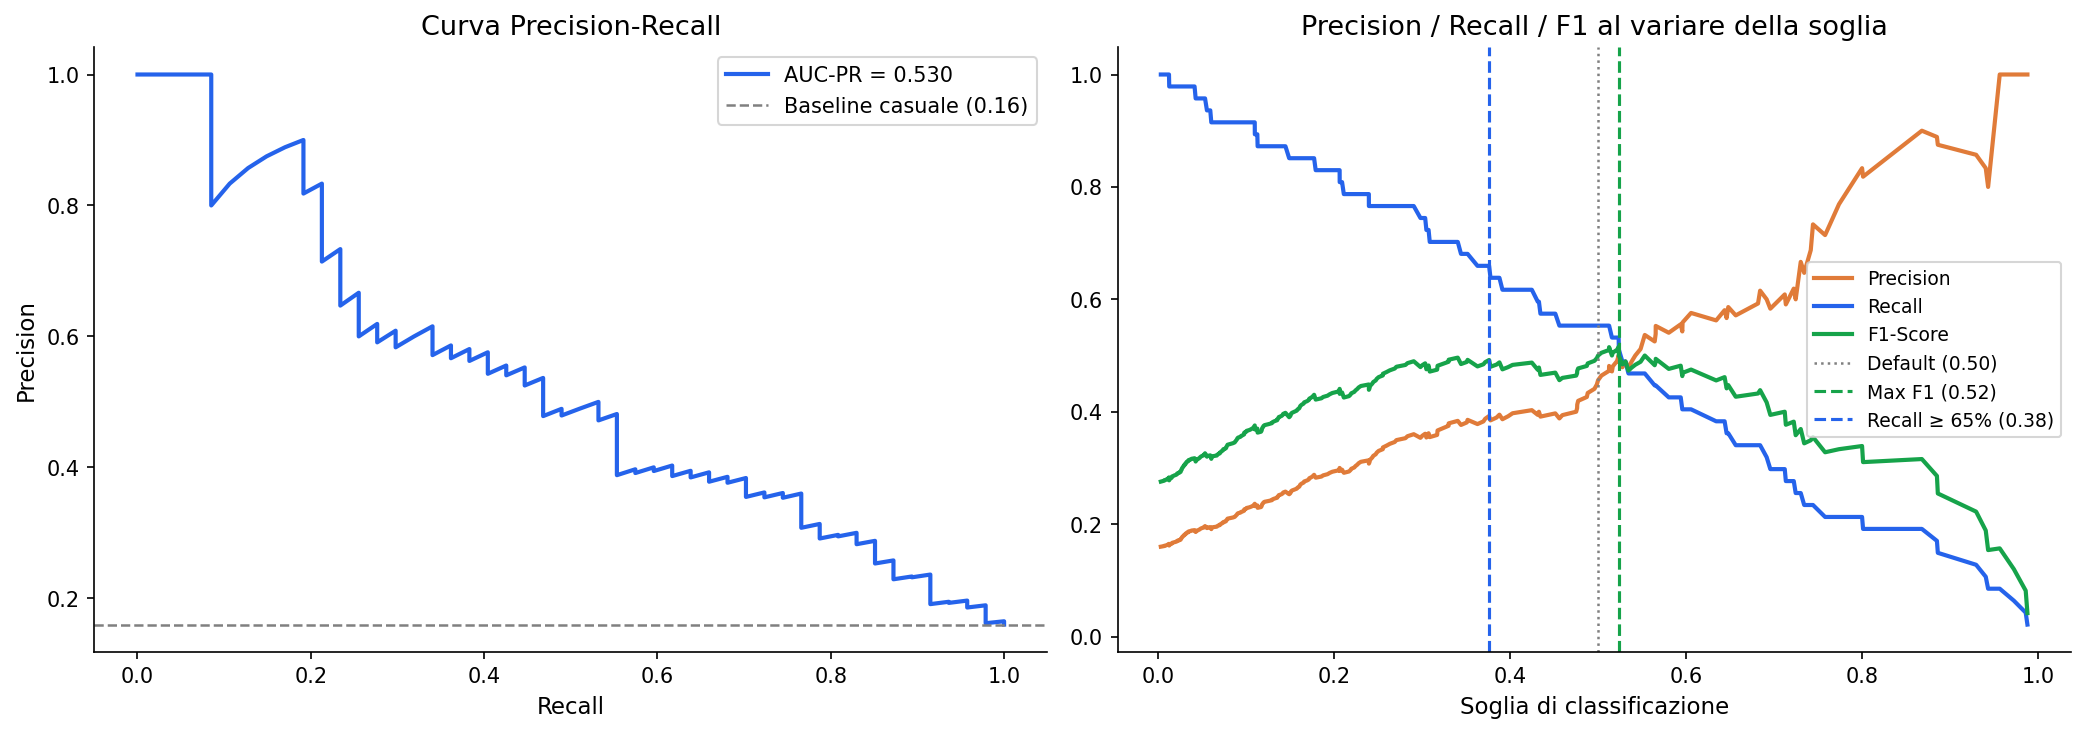
\includegraphics[width=\textwidth]{media/threshold_optimization.png}
    \caption{Ottimizzazione della soglia: curva precision-recall (sinistra) e andamento di precision, recall e F1 in funzione della soglia (destra).}
    \label{fig:threshold_optimization}
\end{figure}

La soglia business-oriented implementa operativamente il principio secondo cui, nel contesto HR, il recall conta più della precision. L'interpretazione è che il modello, in produzione, dovrebbe essere tarato per essere \emph{prudente}: preferibile segnalare qualche caso in più alla verifica dell'HR manager piuttosto che lasciarsi sfuggire un dipendente realmente a rischio. Questo è un punto di contatto tra la componente predittiva e la componente esplicativa della pipeline: una soglia più bassa aumenta la quantità di istanze per cui si genereranno spiegazioni locali, il che rende ancora più importante disporre di strumenti di XAI capaci di distinguere, \emph{a posteriori}, tra segnalazioni solide e segnalazioni borderline.

\section{Spiegazioni SHAP}
\label{sec:shap}

SHAP è stato applicato nella variante \texttt{TreeExplainer}, che sfrutta la struttura del modello XGBoost per calcolare in modo esatto i valori di Shapley in tempo polinomiale. Questa scelta offre due garanzie rilevanti: \emph{model-awareness} (i valori sono coerenti con la decisione effettiva del modello, non con un'approssimazione surrogata) e \emph{determinismo} (non essendoci campionamento, ripetizioni successive producono gli stessi risultati). Entrambe le proprietà sono desiderabili in un contesto HR, dove la riproducibilità delle spiegazioni è una precondizione per il loro utilizzo all'interno di processi decisionali.

\subsection{Importanza globale delle feature}

L'aggregazione dei valori SHAP assoluti sull'intero test set fornisce una misura di importanza globale, visualizzata come summary plot in Figura~\ref{fig:shap_summary}. Ogni riga rappresenta una feature, ordinata per contributo medio assoluto, e ogni punto un dipendente; il colore indica il valore della feature, mentre la posizione orizzontale indica l'impatto SHAP sulla predizione.

\begin{figure}[htbp]
    \centering
    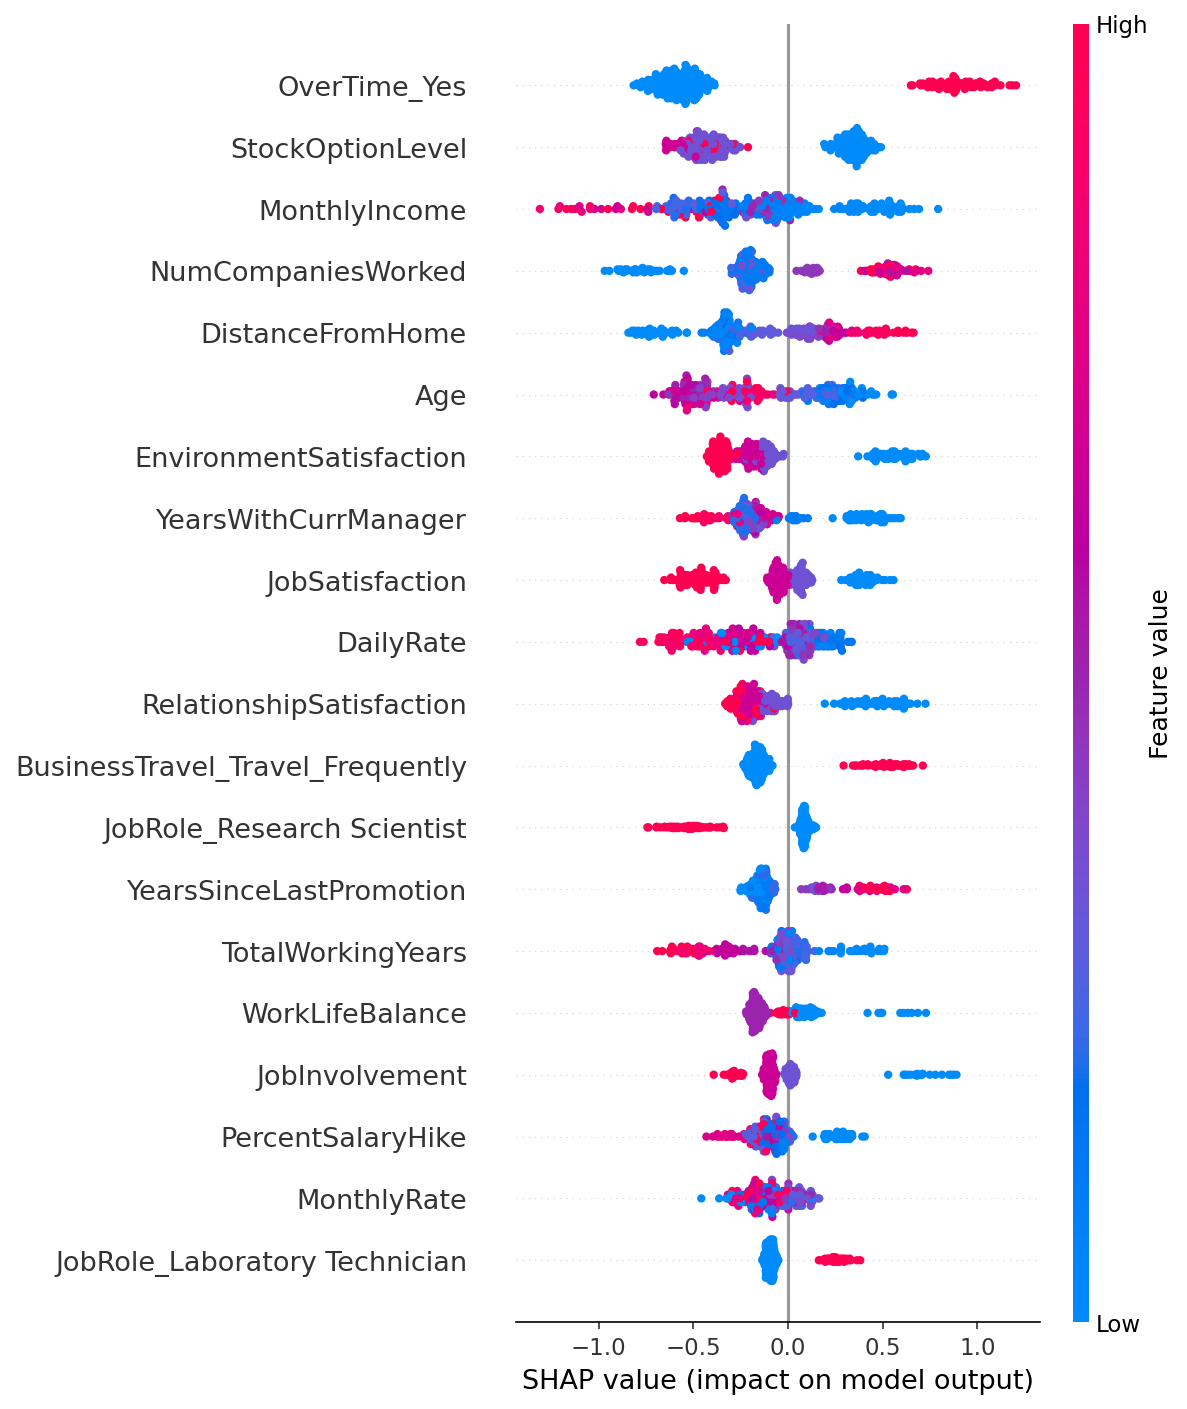
\includegraphics[width=0.85\textwidth]{media/shap_summary_plot.png}
    \caption{SHAP summary plot sul test set: ranking globale delle feature per impatto medio assoluto sulla predizione.}
    \label{fig:shap_summary}
\end{figure}

Le feature che emergono nelle prime posizioni sono coerenti con la letteratura HR riportata nel Capitolo~\ref{cap:quadro_teorico}: \texttt{OverTime\_Yes}, \texttt{MonthlyIncome}, \texttt{StockOptionLevel}, \texttt{JobSatisfaction} e le variabili di tenure compaiono come i principali driver. La lettura del grafico è duplice: da un lato il summary plot sintetizza \emph{quali} feature pesano sul modello in aggregato, dall'altro rende esplicito il \emph{verso} del loro impatto. Valori alti di \texttt{OverTime\_Yes} (cioè la presenza di straordinari) si associano a contributi SHAP positivi, spostando la predizione verso la classe ``abbandono''. Valori alti di \texttt{MonthlyIncome} o \texttt{StockOptionLevel}, al contrario, si associano a contributi negativi.

Questa vista aggregata è utile per ottenere una comprensione d'insieme del modello, ma non è sufficiente per supportare una decisione su un singolo dipendente: per quest'ultimo scopo occorre passare alle spiegazioni locali.

\subsection{Tre casi locali: vero positivo, falso positivo, falso negativo}

Per illustrare l'utilità operativa di SHAP e per disporre di un paniere comune da confrontare con LIME e con i controfattuali, sono stati selezionati tre dipendenti rappresentativi di situazioni diverse rispetto al modello. La selezione non è casuale: si tratta di un vero positivo con probabilità elevata (Dip.~214), un falso positivo con probabilità elevata (Dip.~223) e un falso negativo (Dip.~240), cioè un dipendente realmente uscito che il modello ha però classificato come stabile. I tre casi permettono di esplorare, rispettivamente, la situazione in cui il modello è corretto e le due modalità principali in cui può sbagliare.

\paragraph{Dipendente~214 --- Vero Positivo.} Il modello attribuisce a questo dipendente una probabilità di abbandono pari al \num{96{,}7}\%, e in effetti il dipendente ha lasciato l'azienda. Il waterfall plot in Figura~\ref{fig:shap_wf_214} mostra come si arrivi a tale predizione a partire dal valore atteso. I contributi dominanti sono tutti nella medesima direzione, cioè di rinforzo del rischio: \texttt{OverTime\_Yes} (presenza di straordinari), valori bassi di \texttt{JobSatisfaction} e \texttt{EnvironmentSatisfaction}, una tenure recente con il manager corrente, un reddito relativamente basso rispetto al livello di ruolo. Il quadro complessivo è quello di un profilo su cui molteplici fattori di rischio si sommano, ciascuno dei quali potenzialmente \emph{intervenibile} da parte dell'HR (sui turni, sulla mobilità interna, sulla retribuzione). È un caso in cui la predizione è sia corretta sia azionabile: lo strumento funziona.

\begin{figure}[htbp]
    \centering
    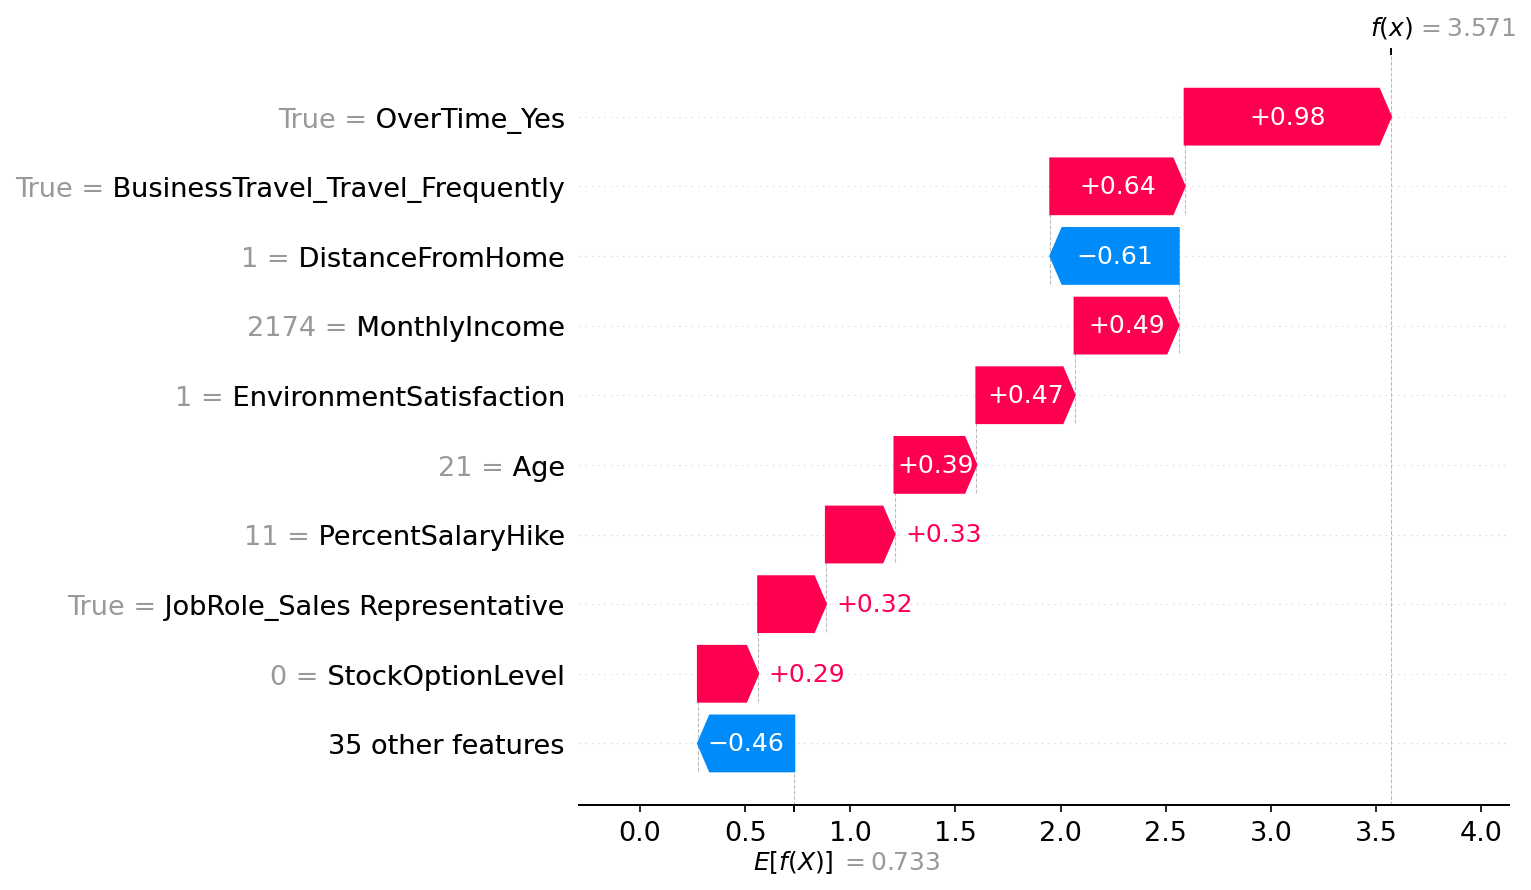
\includegraphics[width=\textwidth]{media/shap_waterfall_emp214_true_positive.png}
    \caption{SHAP waterfall plot per il Dipendente~214 (vero positivo, $P(\text{Left})=0{,}967$).}
    \label{fig:shap_wf_214}
\end{figure}

\paragraph{Dipendente~223 --- Falso Positivo.} Il modello predice un'elevata probabilità di abbandono ($\approx\num{86{,}1}\%$), ma il dipendente è in realtà rimasto. Il waterfall plot in Figura~\ref{fig:shap_wf_223} mostra un profilo per molti versi simile al precedente: presenza di straordinari, stock option assenti, reddito contenuto. La differenza con il caso~214 sta nel fatto che alcune di queste variabili descrivono una condizione transitoria tipica di chi è all'inizio della carriera (giovane, da poco in azienda, retribuzione coerente con il livello), che il modello interpreta come segnale di instabilità ma che non necessariamente preannuncia un abbandono. In altri termini, il modello tende a sovrastimare il peso della componente retributiva e di tenure per i profili più giovani. È un promemoria utile del fatto che, anche quando il modello è ``sicuro'' (probabilità alta), la predizione può essere errata se il contesto del dipendente è al di fuori della distribuzione su cui il modello è stato tarato.

\begin{figure}[htbp]
    \centering
    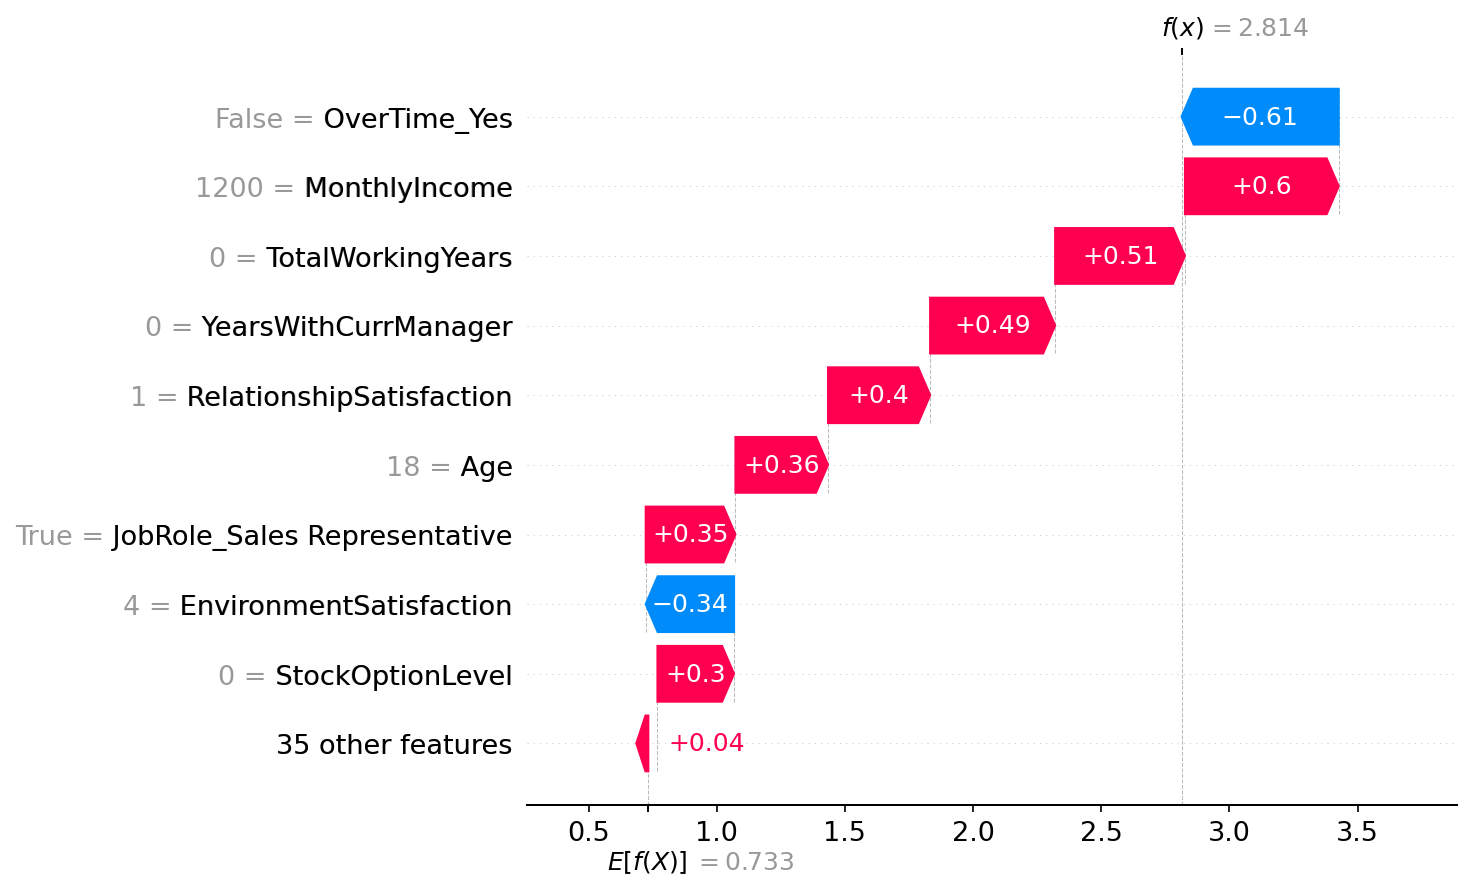
\includegraphics[width=\textwidth]{media/shap_waterfall_emp223_false_positive.png}
    \caption{SHAP waterfall plot per il Dipendente~223 (falso positivo, $P(\text{Left})=0{,}861$).}
    \label{fig:shap_wf_223}
\end{figure}

\paragraph{Dipendente~240 --- Falso Negativo.} Il modello attribuisce a questo dipendente una probabilità di abbandono pressoché nulla ($\approx\num{0{,}7}\%$), eppure il dipendente ha lasciato l'azienda. Il waterfall plot in Figura~\ref{fig:shap_wf_240} mostra come quasi tutti i contributi SHAP siano negativi (cioè favorevoli alla permanenza): soddisfazione alta, assenza di straordinari, tenure consolidata, retribuzione elevata. Sulla base delle sole feature osservabili nel dataset il profilo è un profilo di permanenza tipico; il fatto che il dipendente sia invece uscito suggerisce che la decisione sia stata guidata da fattori \emph{non contenuti nel dataset} --- un'offerta esterna, una trasformazione personale, un conflitto specifico con il team --- che nessuna spiegazione locale basata sulle feature disponibili può recuperare. Il falso negativo non è quindi un errore del metodo di spiegazione ma un \emph{limite intrinseco del dataset}, ed è un caso utile per formare l'utente finale sull'idea che il sistema supporta la decisione umana ma non la sostituisce.

\begin{figure}[htbp]
    \centering
    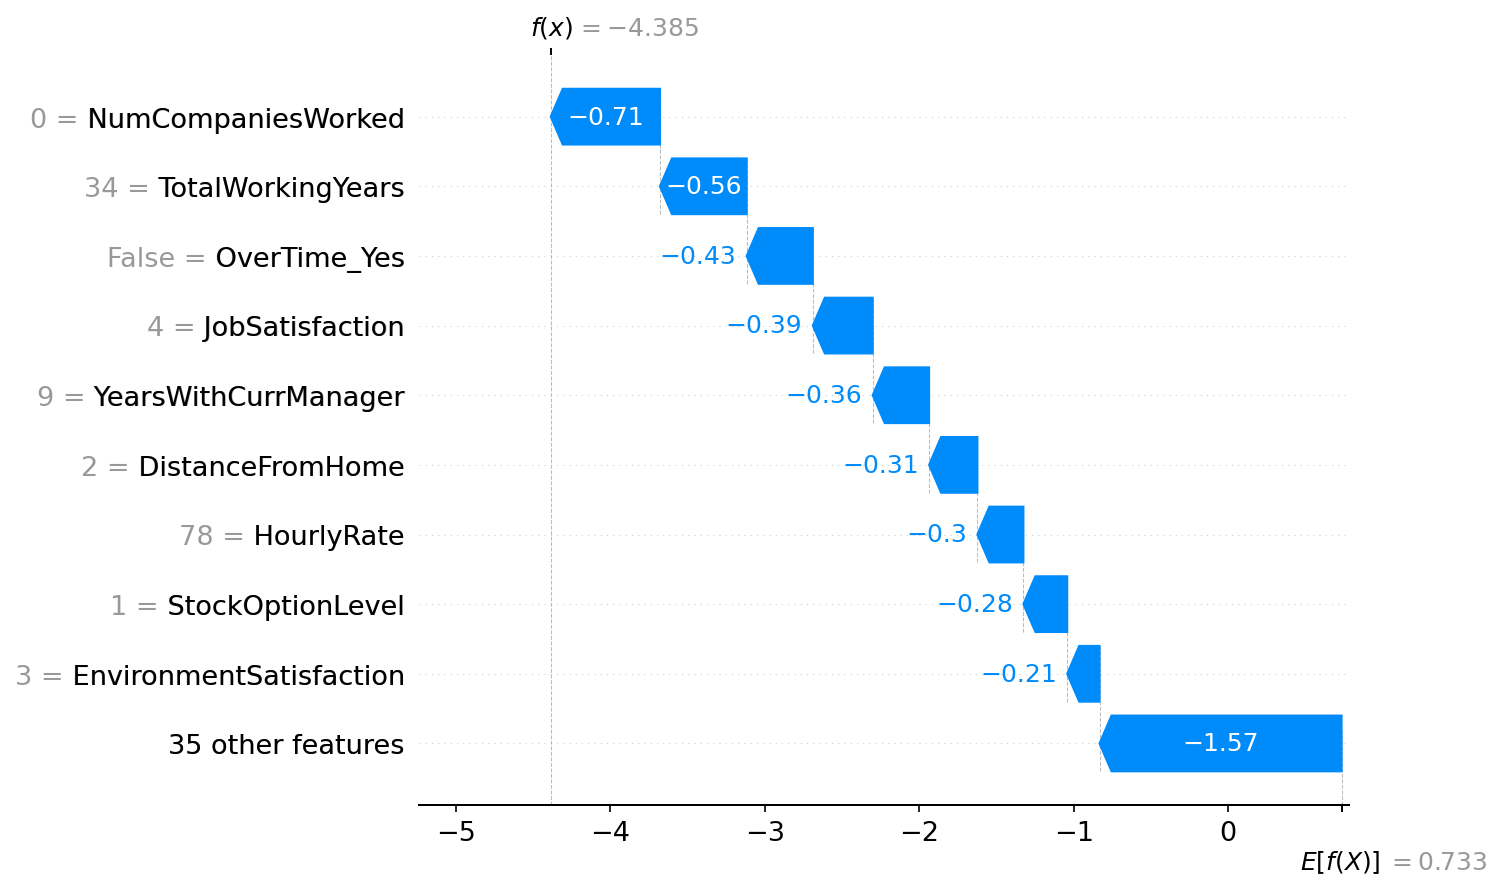
\includegraphics[width=\textwidth]{media/shap_waterfall_emp240_false_negative.png}
    \caption{SHAP waterfall plot per il Dipendente~240 (falso negativo, $P(\text{Left})=0{,}007$).}
    \label{fig:shap_wf_240}
\end{figure}

La triade di casi mostra come SHAP sia in grado di fornire una narrazione coerente anche quando il modello sbaglia: la spiegazione locale è parte integrante della diagnosi, non solo della validazione.

\section{Spiegazioni LIME}
\label{sec:lime}

La seconda famiglia di spiegazioni è stata ottenuta con LIME, nella variante \texttt{LimeTabularExplainer} per dati tabulari. La configurazione utilizzata prevede \texttt{num\_samples=8000} (campioni perturbati per ciascuna spiegazione locale), \texttt{discretize\_continuous=True} (per ottenere spiegazioni in forma di regole su intervalli di valori, più leggibili per un utente non tecnico) e \texttt{random\_state=42}. L'explainer è stato inizializzato sul \emph{training set} per assicurare che la stima della distribuzione di ciascuna feature sia coerente con quella usata dal modello in fase di training.

Rispetto a SHAP, LIME è model-agnostic e basato su un surrogato lineare locale: questa scelta comporta maggiore flessibilità ma anche una dipendenza dalla procedura di campionamento. In questa implementazione il tempo di generazione delle spiegazioni sull'intero test set è risultato di circa \num{39} secondi (\num{294} istanze, $\approx 7{,}43$ istanze al secondo): un ordine di grandezza compatibile con un utilizzo interattivo, ma superiore a quello richiesto dal \texttt{TreeExplainer} di SHAP.

\subsection{Importanza globale aggregata}

Per ottenere una misura di importanza globale da LIME, i pesi locali di ciascuna feature sono stati aggregati in valore assoluto e mediati sulle \num{294} istanze del test set. Il ranking risultante è mostrato in Figura~\ref{fig:lime_global}.

\begin{figure}[htbp]
    \centering
    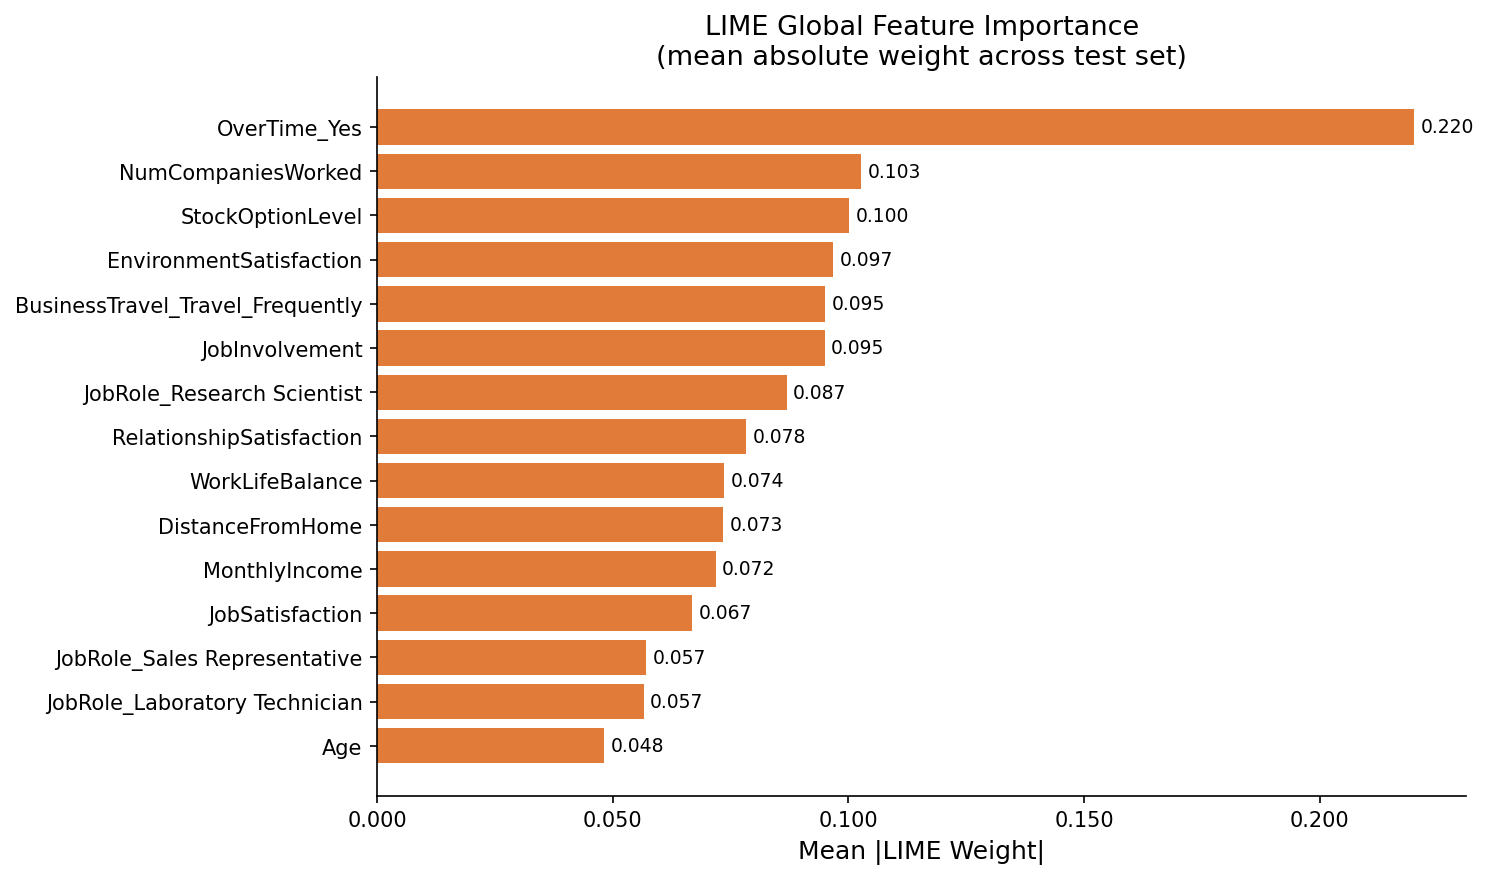
\includegraphics[width=0.85\textwidth]{media/lime_global_feature_importance.png}
    \caption{Ranking globale aggregato delle feature secondo LIME (media dei pesi in valore assoluto sul test set).}
    \label{fig:lime_global}
\end{figure}

Le prime posizioni del ranking LIME ricalcano in larga parte quelle di SHAP: \texttt{OverTime\_Yes} è, anche qui, la feature dominante, seguita da \texttt{BusinessTravel\_Frequently}, \texttt{JobRole\_Research\_Scientist}, \texttt{NumCompaniesWorked} e \texttt{StockOptionLevel}. Le differenze più evidenti rispetto a SHAP riguardano la discretizzazione: LIME, trasformando le feature continue in intervalli, tende ad amplificare il peso delle variabili categoriche o categoriche ottenute \emph{per binning}, mentre SHAP le tratta in forma continua. Questo spiega in parte la maggiore presenza di feature one-hot nelle prime posizioni del ranking LIME.

\subsection{Spiegazioni locali sui tre casi}

L'analisi locale è stata condotta sugli stessi tre dipendenti discussi nella Sezione~\ref{sec:shap}. Le Figure~\ref{fig:lime_local_214}, \ref{fig:lime_local_223} e \ref{fig:lime_local_240} mostrano le spiegazioni LIME per Dip.~214, 223 e 240 rispettivamente.

\begin{figure}[htbp]
    \centering
    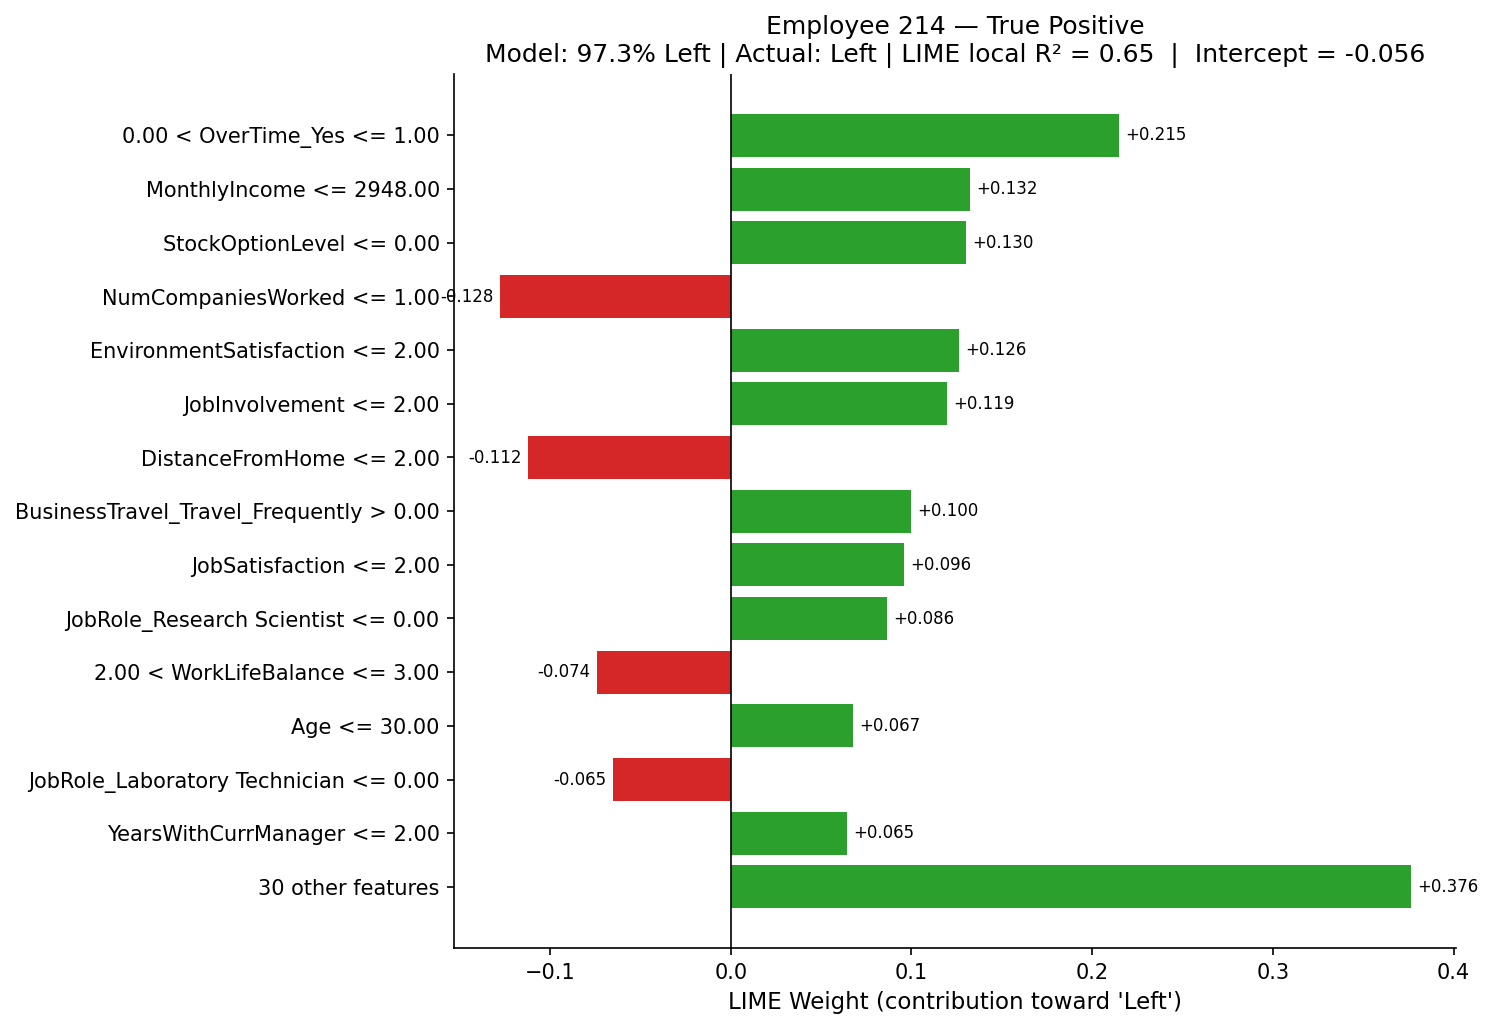
\includegraphics[width=\textwidth]{media/lime_local_emp214_true_positive.png}
    \caption{LIME local explanation per il Dipendente~214.}
    \label{fig:lime_local_214}
\end{figure}

\begin{figure}[htbp]
    \centering
    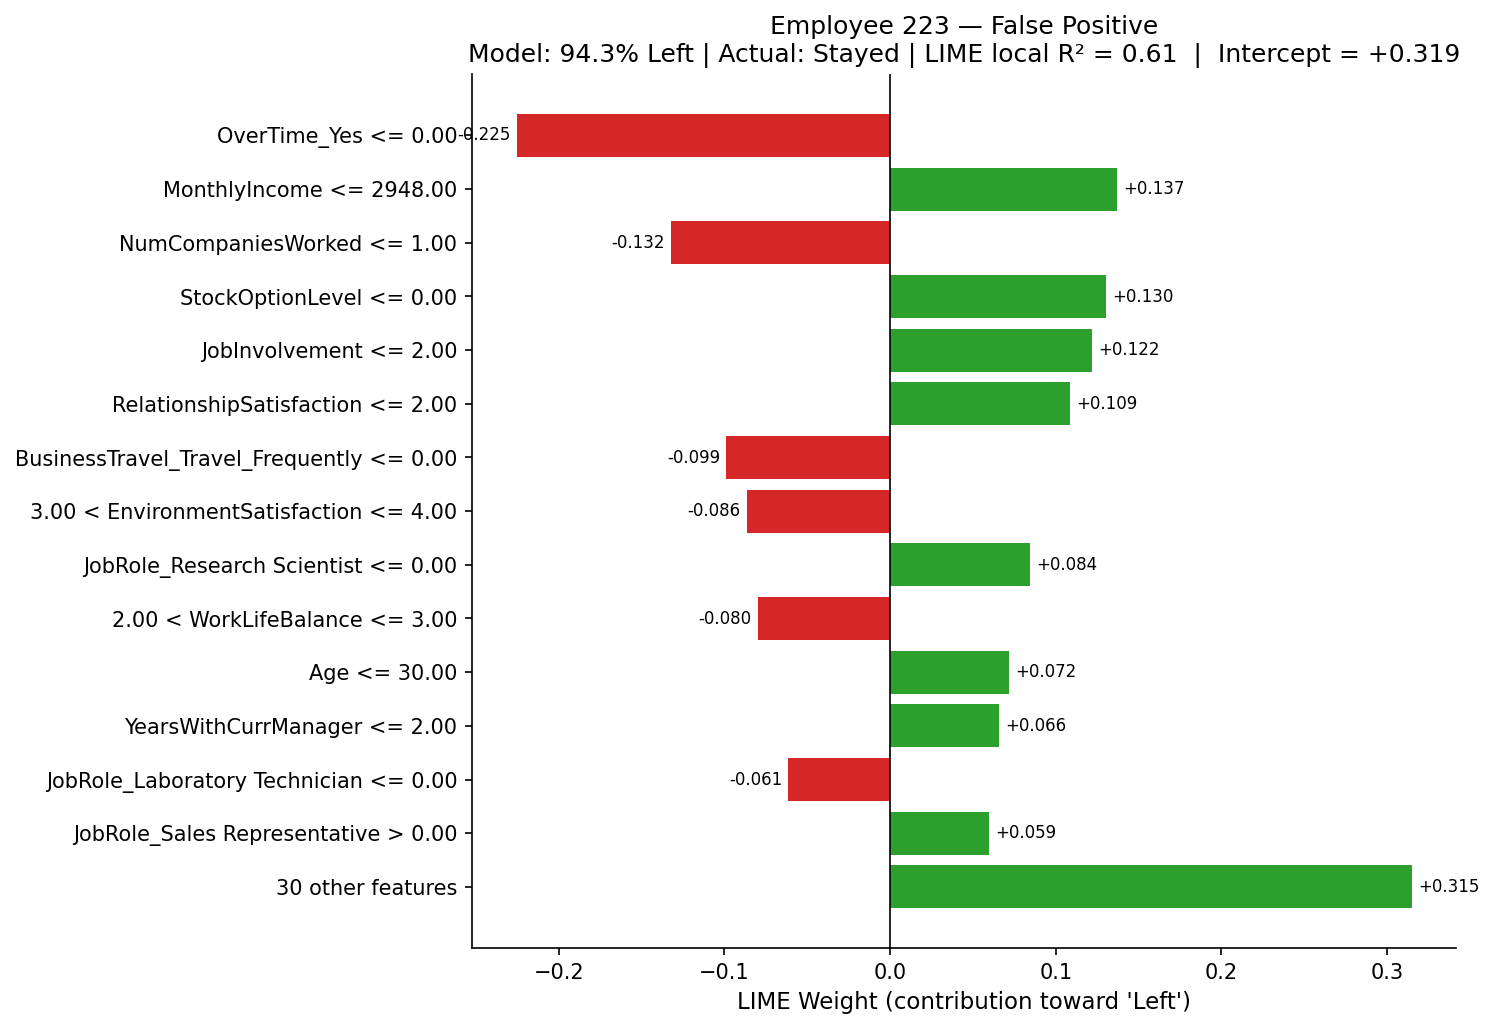
\includegraphics[width=\textwidth]{media/lime_local_emp223_false_positive.png}
    \caption{LIME local explanation per il Dipendente~223.}
    \label{fig:lime_local_223}
\end{figure}

\begin{figure}[htbp]
    \centering
    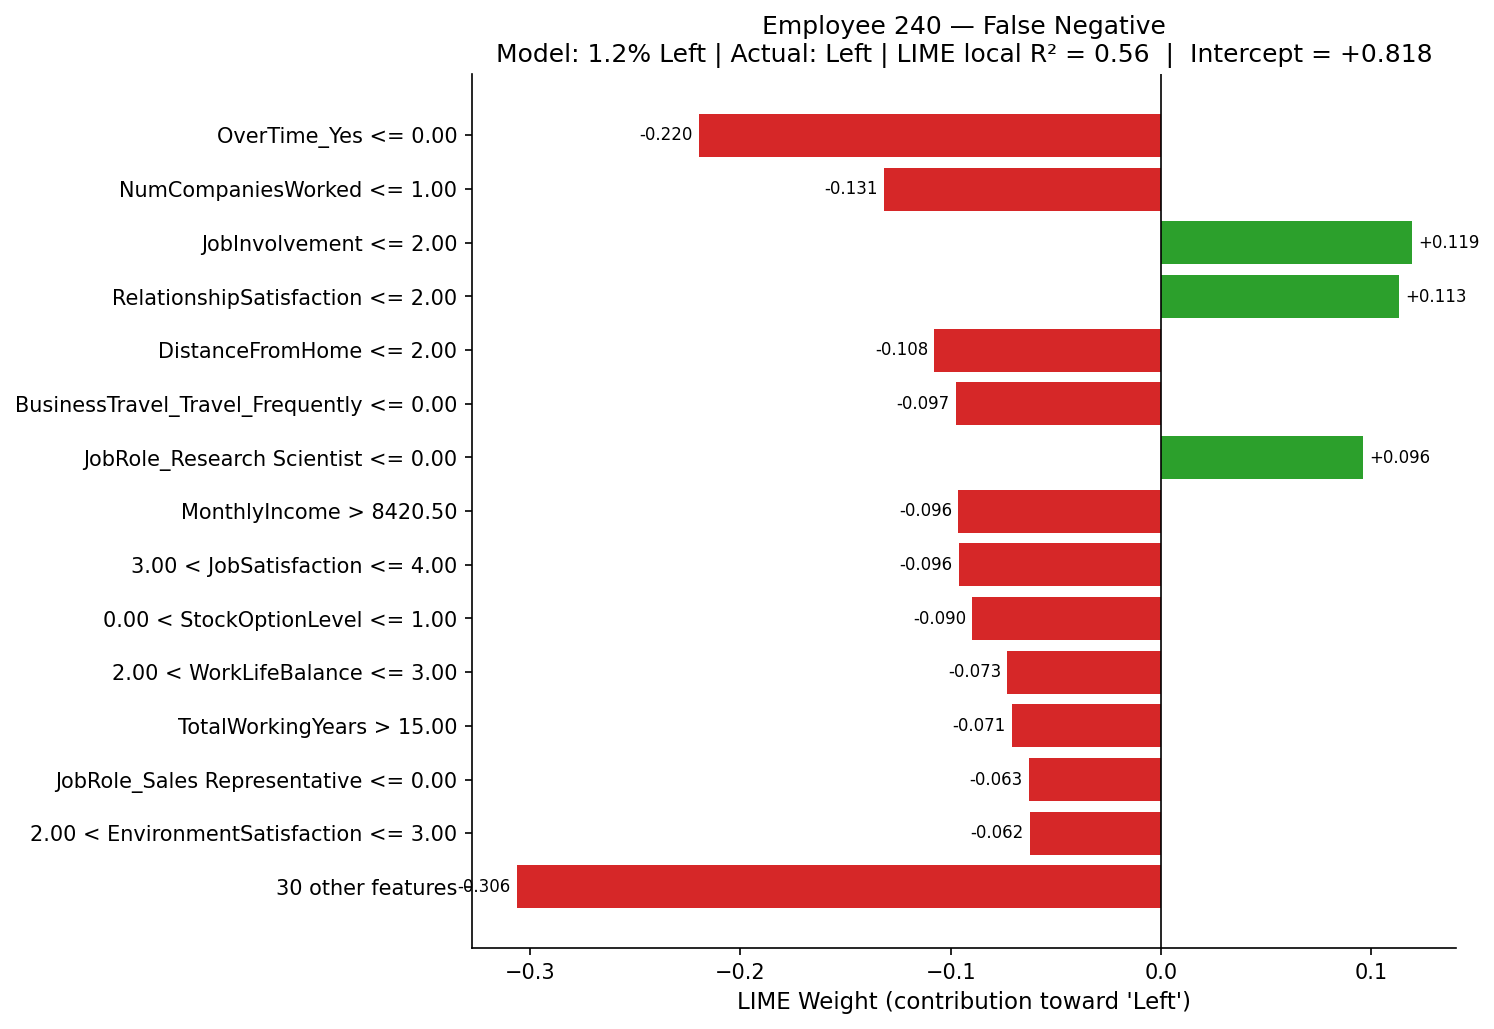
\includegraphics[width=\textwidth]{media/lime_local_emp240_false_negative.png}
    \caption{LIME local explanation per il Dipendente~240.}
    \label{fig:lime_local_240}
\end{figure}

Per il Dip.~214 il quadro è sostanzialmente concorde con quello di SHAP: \texttt{OverTime\_Yes} è il principale driver di rischio, insieme all'assenza di stock option e a un reddito al di sotto di una soglia di riferimento. Per il Dip.~223 LIME attribuisce un ruolo ancor più marcato alla retribuzione e alla bassa tenure, rendendo esplicito il pattern del ``profilo giovane'' già individuato da SHAP. Per il Dip.~240 LIME, come SHAP, riporta un quadro di sostanziale stabilità: le feature osservate non contengono segnali di uscita, e il modello di spiegazione riflette fedelmente questa assenza.

Un aspetto da sottolineare è la presenza di discordanze puntuali tra i due metodi: alcune feature che SHAP considera rilevanti perdono peso in LIME e viceversa. Questo non indica un errore di uno dei due metodi, ma la diversa natura delle spiegazioni: SHAP attribuisce in modo additivo la differenza tra la predizione del modello e il suo valore atteso, mentre LIME approssima localmente la superficie di decisione con un modello lineare. In presenza di feature fortemente correlate (come le variabili di tenure) o di effetti non lineari locali, le due prospettive possono produrre ranking diversi pur spiegando lo stesso fenomeno.

\subsection{Confronto sinottico}

Per rendere esplicite le differenze strutturali tra i due framework, la Figura~\ref{fig:shap_vs_lime} riporta un confronto sinottico delle due metodologie lungo gli assi rilevanti per l'uso applicativo.

\begin{figure}[htbp]
    \centering
    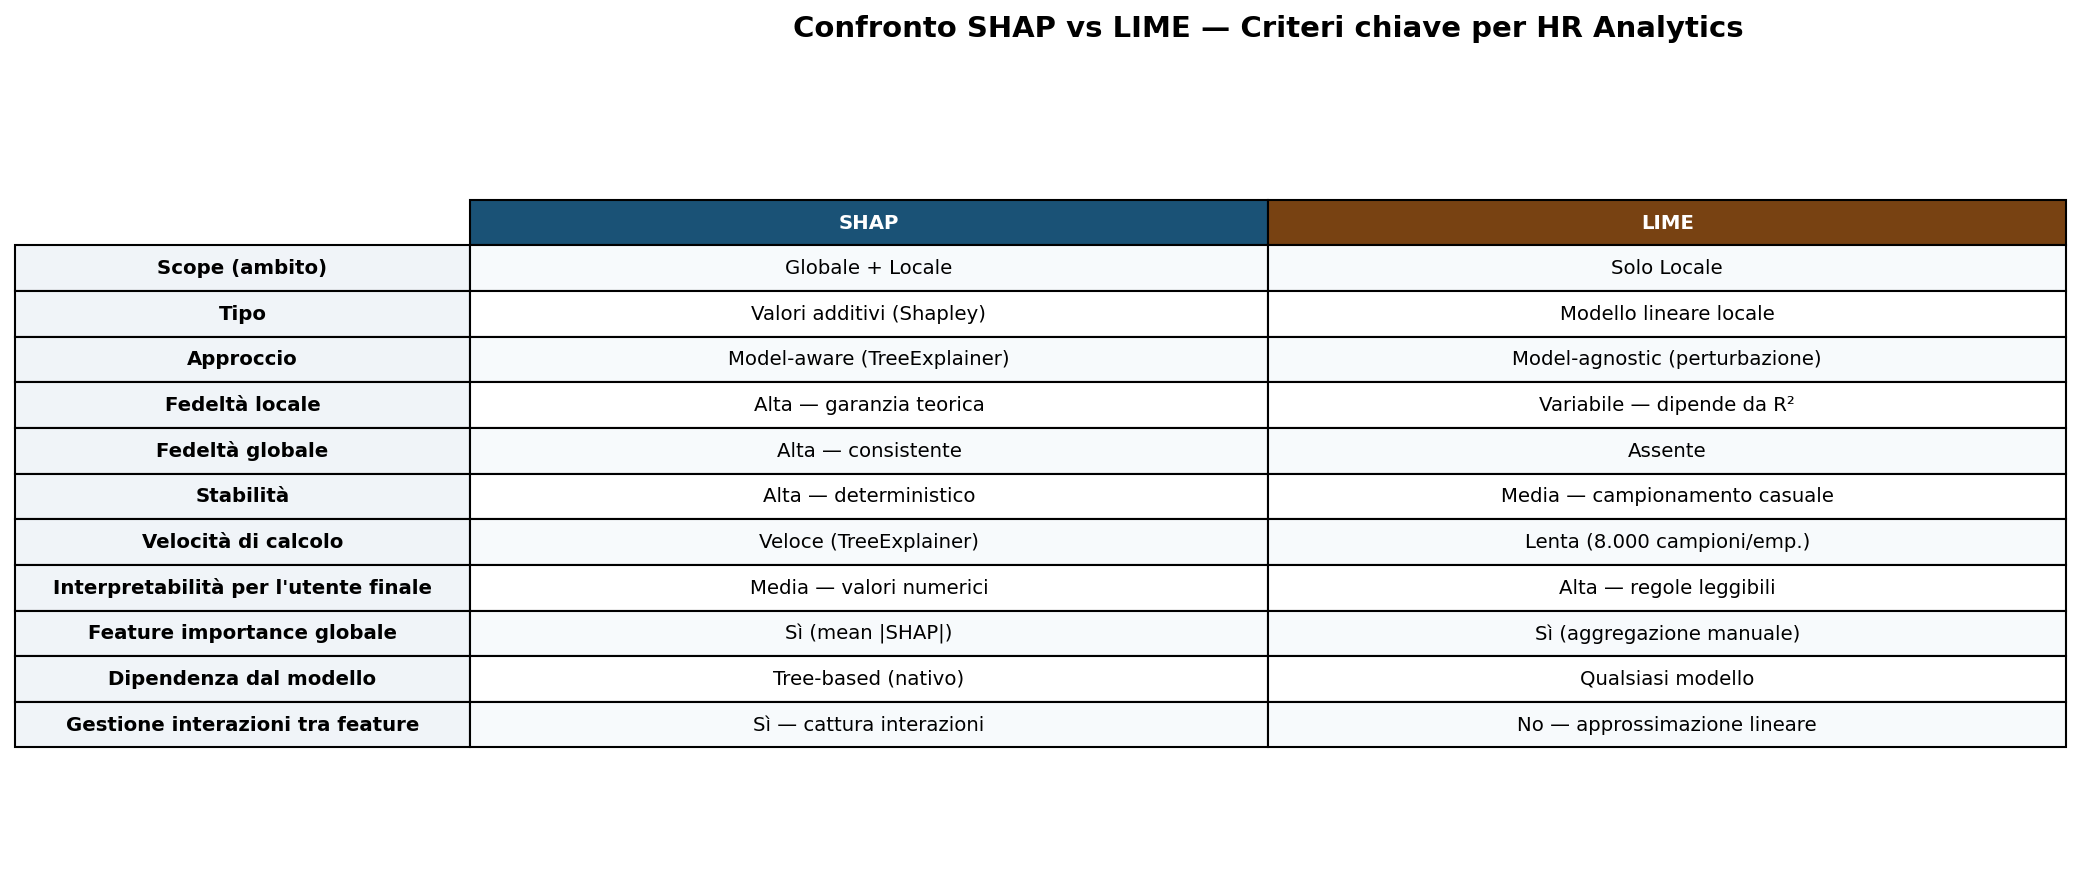
\includegraphics[width=0.95\textwidth]{media/shap_vs_lime_comparison.png}
    \caption{Confronto sinottico SHAP vs LIME: ambito, fedeltà, stabilità, velocità, dipendenza dal modello.}
    \label{fig:shap_vs_lime}
\end{figure}

Dal confronto emergono tre indicazioni coerenti con quanto discusso al Capitolo~\ref{cap:quadro_teorico}: SHAP è preferibile quando si cerca una spiegazione \emph{formalmente fondata} e deterministica di un modello ad albero, a fronte di un'integrazione che richiede un \emph{explainer} specifico per l'architettura; LIME è preferibile quando è importante ottenere spiegazioni sotto forma di regole discretizzate, potenzialmente più vicine al linguaggio di un utente HR, e quando il modello sottostante è sostituibile o non trattabile tramite explainer dedicati. Nel caso studio entrambi i metodi producono, sugli stessi tre dipendenti, narrazioni sovrapponibili: le discordanze sono locali e riconducibili a caratteristiche note dei due approcci, non a errori.

\section{Analisi controfattuale (Alibi)}
\label{sec:alibi}

SHAP e LIME rispondono alla domanda \emph{``perché il modello ha deciso così?''}. I controfattuali rispondono invece alla domanda, operativamente più utile per un HR manager, \emph{``cosa dovrebbe cambiare perché il modello decida diversamente?''}. Questa sezione applica la classe \texttt{CounterfactualProto} della libreria Alibi ai due dipendenti classificati come ad alto rischio (Dip.~214 e Dip.~223), per verificare in che misura il controfattuale restituisca suggerimenti operativi coerenti con quanto già osservato nelle spiegazioni attribuitive.

\subsection{Configurazione dell'explainer}

L'explainer è stato configurato con la variante basata su prototipi guidati da \texttt{k-d tree} (in alternativa all'autoencoder), scelta che riduce il tempo di ottimizzazione e non richiede un modello generativo ausiliario. I parametri principali della funzione obiettivo sono stati fissati come segue: \texttt{kappa}\,$=0{,}1$ (margine della loss di classificazione), \texttt{beta}\,$=0{,}1$ (peso della regolarizzazione $L_1$, responsabile della \emph{sparsity} del controfattuale), \texttt{theta}\,$=10$ (peso del termine di prossimità al prototipo di classe, che garantisce \emph{plausibilità}), \texttt{gamma}\,$=100$ (peso della regolarizzazione $L_2$) e \texttt{max\_iter}\,$=500$. Il \texttt{feature\_range} è stato derivato dai valori minimo e massimo osservati sul training set, per evitare che l'ottimizzatore proponga valori al di fuori del dominio empirico. I dati sono stati convertiti in \texttt{float32} prima di essere passati all'explainer; le piccole differenze numeriche tra le probabilità riportate qui e quelle di SHAP derivano da questa conversione.

\subsection{Dipendente~214: una lettura operativa coerente}

Il controfattuale per il Dip.~214 porta la probabilità di abbandono stimata dal modello da $\approx \num{97{,}3}\%$ a $\approx \num{24{,}6}\%$, un calo che attraversa la soglia di decisione. I cambiamenti suggeriti (Figura~\ref{fig:cf_214}) convergono su un insieme coerente di leve: rimozione degli straordinari (\texttt{OverTime}), riduzione della frequenza dei viaggi di lavoro, aumento della permanenza col manager corrente, aumento del coinvolgimento nel ruolo e aumento della frequenza della formazione.

\begin{figure}[htbp]
    \centering
    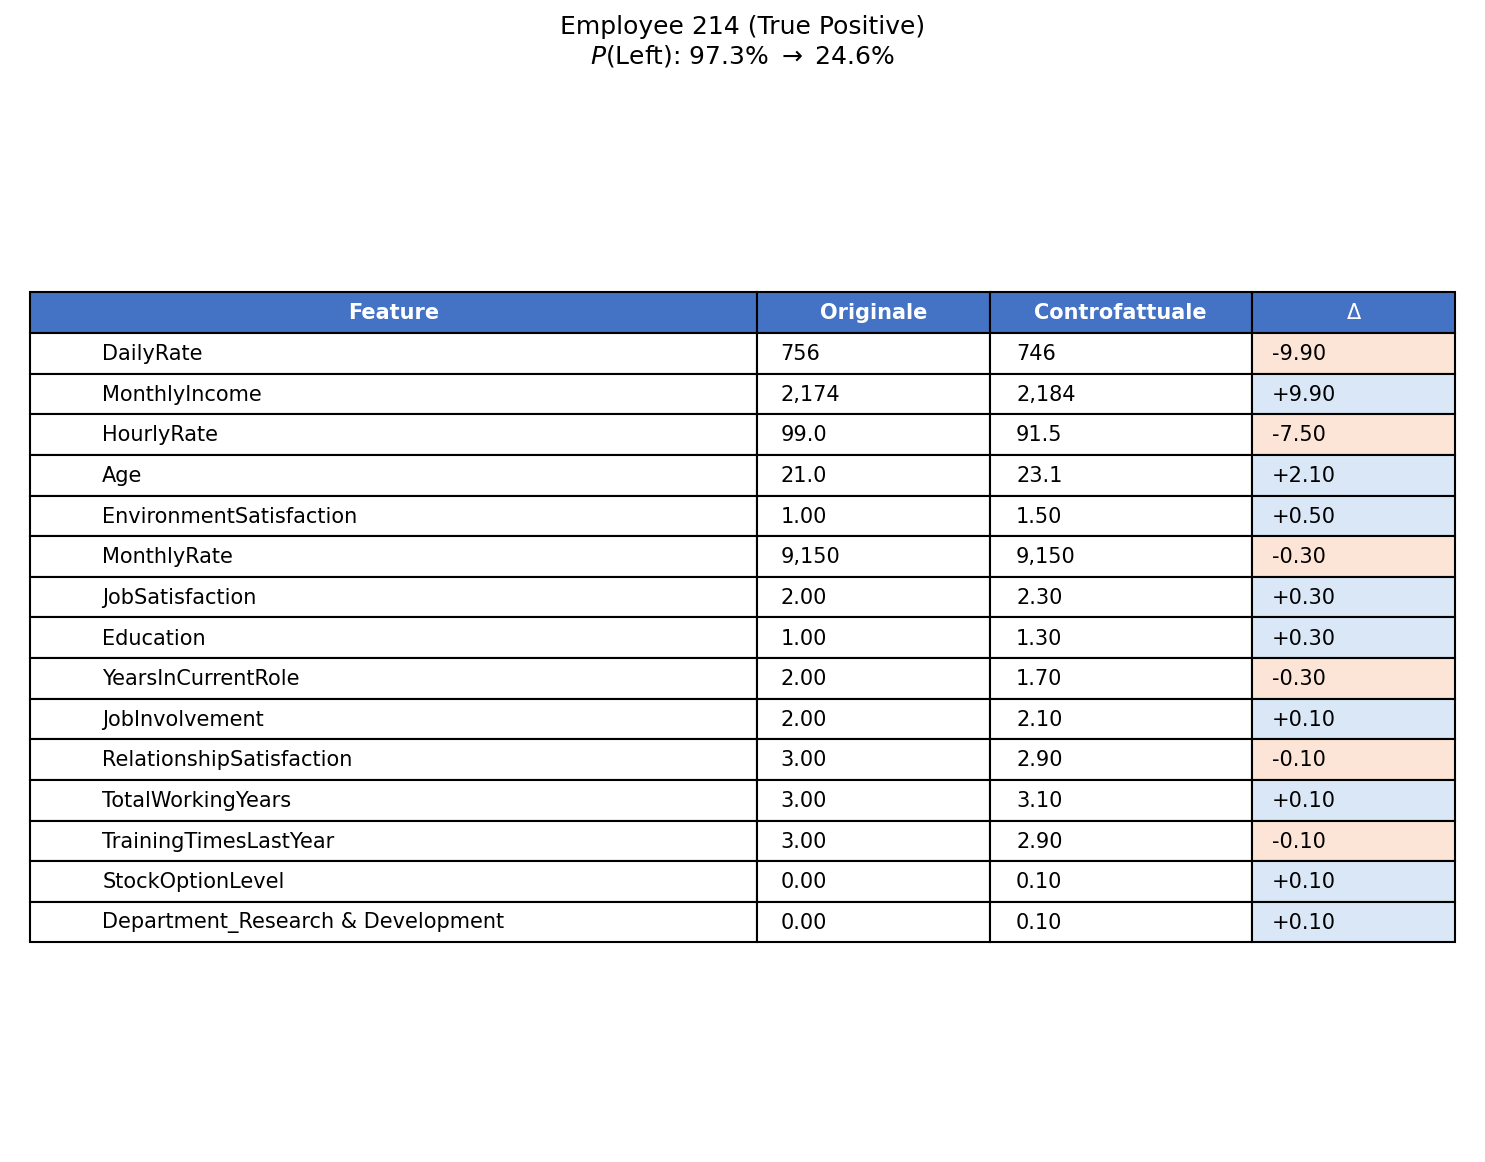
\includegraphics[width=0.95\textwidth]{media/cf_emp214_true_positive.png}
    \caption{Controfattuale per il Dipendente~214: feature modificate dall'ottimizzatore con variazione tra valore originale e valore controfattuale.}
    \label{fig:cf_214}
\end{figure}

L'aspetto operativamente rilevante è che queste leve sono, in buona parte, \emph{azionabili} da un'organizzazione: una revisione del carico di lavoro, un piano di mobilità interna, un investimento in formazione sono interventi reali di politica del personale. Il controfattuale, in questo caso, non solo concorda con la diagnosi fornita da SHAP e LIME (che indicavano \texttt{OverTime} come fattore dominante di rischio), ma estende la spiegazione in direzione prescrittiva: \emph{dato} il profilo del dipendente, quali combinazioni di interventi avrebbero portato la predizione al di sotto della soglia di rischio.

\subsection{Dipendente~223: un controfattuale che rivela bias del modello}

Il controfattuale per il Dip.~223 porta la probabilità stimata da $\approx\num{94{,}3}\%$ a $\approx\num{41{,}6}\%$: la riduzione è netta, ma non sufficiente a incrociare la soglia di decisione nella sua accezione più conservativa. Il punto di interesse non è tanto il valore finale quanto la \emph{natura} dei cambiamenti suggeriti (Figura~\ref{fig:cf_223}): l'ottimizzatore propone in particolare un incremento sensibile dell'età (da \num{18} a circa \num{30} anni), una riduzione della distanza da casa e un aumento dell'anzianità in azienda e nel ruolo corrente.

\begin{figure}[htbp]
    \centering
    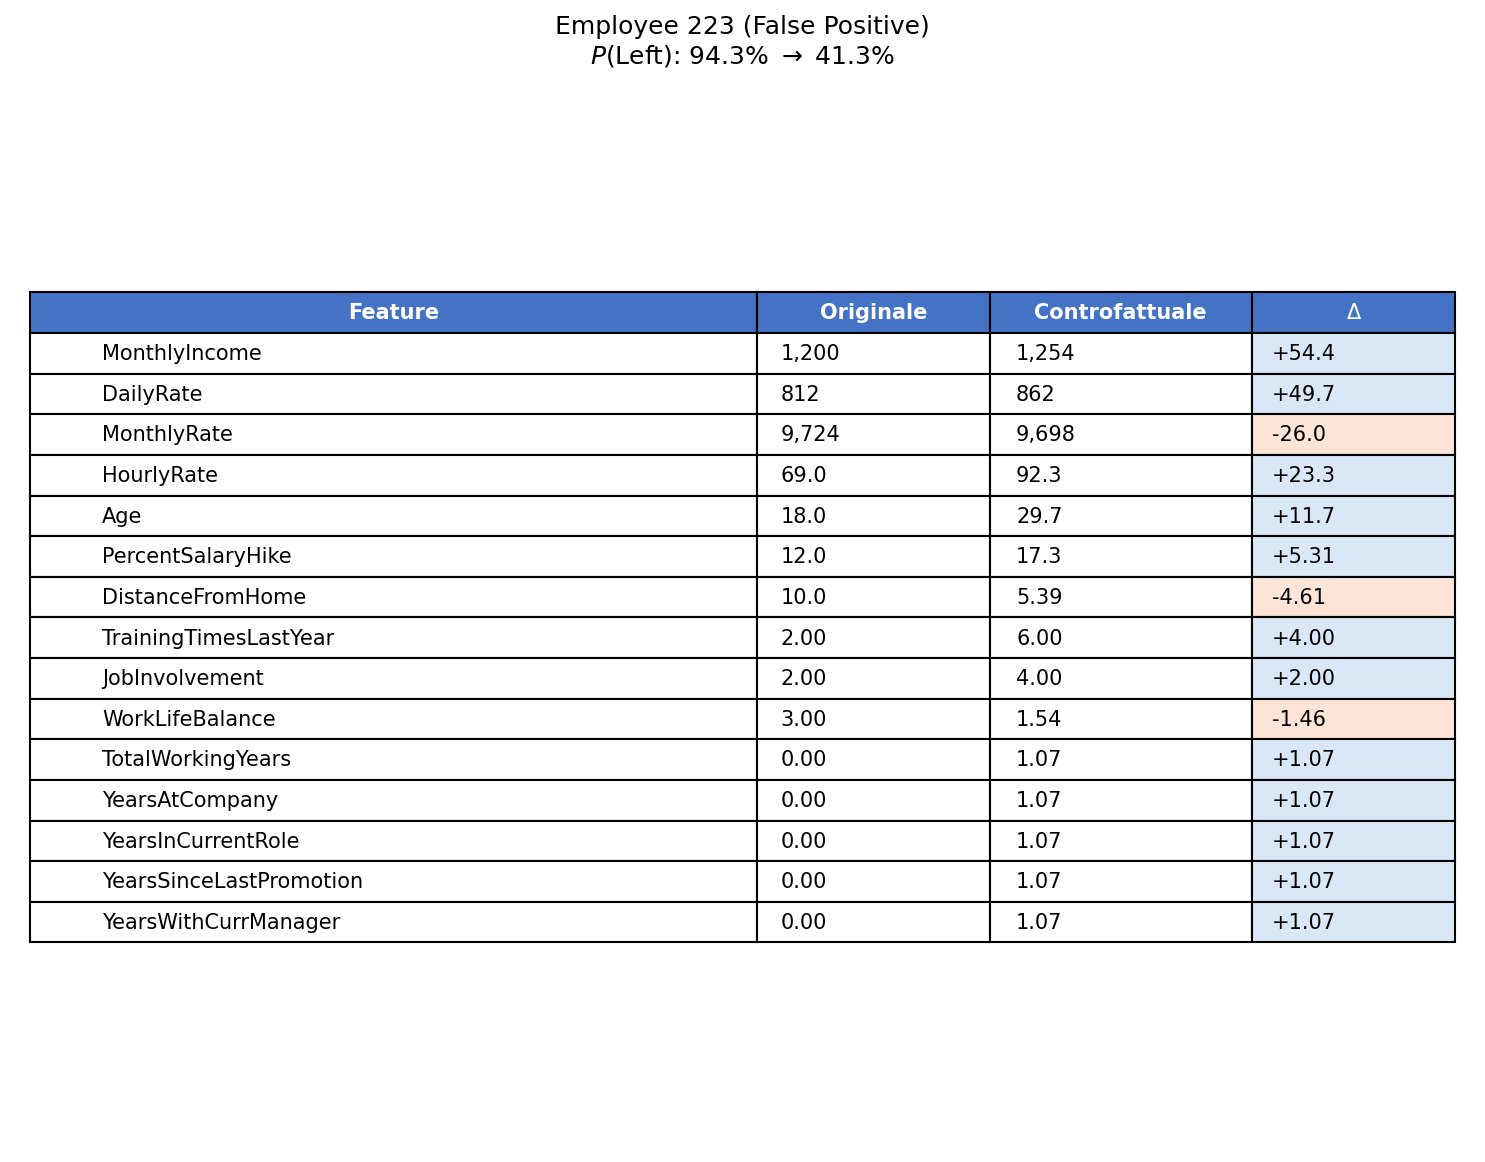
\includegraphics[width=0.95\textwidth]{media/cf_emp223_false_positive.png}
    \caption{Controfattuale per il Dipendente~223: l'ottimizzatore propone modifiche su variabili demografiche e di tenure, rivelando il bias del modello verso i profili giovani.}
    \label{fig:cf_223}
\end{figure}

Queste modifiche hanno due caratteristiche di lettura diverse. Da un lato, rafforzano quanto già osservato nelle sezioni precedenti: il modello attribuisce una quota consistente di rischio al pattern \emph{dipendente giovane, appena assunto, che vive lontano}, e per abbassare la probabilità bisogna di fatto trasformare il dipendente in un profilo diverso. Dall'altro, alcune di queste feature sono \emph{immutabili} o non direttamente azionabili da parte dell'azienda: età, anzianità e distanza da casa non sono leve su cui un HR manager può intervenire. Il controfattuale, in questo caso, non fornisce una prescrizione operativa ma svolge una funzione diagnostica: rende visibile un potenziale bias del modello e segnala che la predizione originaria, pur essendo ``spiegabile'', andrebbe trattata con cautela prima di generare un'azione concreta.

\subsection{Leve azionabili vs fattori immutabili}

I due casi, presi insieme, mostrano che il valore di una spiegazione controfattuale dipende in modo decisivo dalla natura delle feature che entrano nella proposta di modifica. Le feature che possono essere considerate \emph{leve azionabili} in un contesto HR --- tipicamente \texttt{OverTime}, \texttt{StockOptionLevel}, \texttt{TrainingTimesLastYear}, \texttt{BusinessTravel} --- producono controfattuali traducibili in azioni manageriali concrete. Le feature \emph{strutturali o immutabili} --- tipicamente \texttt{Age}, \texttt{TotalWorkingYears}, \texttt{YearsAtCompany}, \texttt{DistanceFromHome} --- producono controfattuali che non sono prescrittivi ma che hanno comunque valore come \emph{test di robustezza} del modello: la loro comparsa in una spiegazione controfattuale segnala che la predizione è sensibile a caratteristiche su cui l'intervento è impossibile o eticamente problematico.

Questa distinzione, assente nelle spiegazioni attributive di SHAP e LIME, è il contributo specifico dei controfattuali al flusso di analisi: non si limita a dire cosa il modello sta guardando, ma forza l'utente a interrogarsi su cosa il modello \emph{dovrebbe} poter guardare in un processo decisionale responsabile.

\section{Dashboard}
\label{sec:dashboard}

% Panoramica sulla dashboard Streamlit (sezione da scrivere in una fase successiva).
